\subsection{Out-of-Sample Behaviour: The Held-Out Year}
\label{Subsection:OutOfSample}

The split of Equation~\ref{Equation:Split} trains on 2015 to 2023, selects among episodes on 2024, and leaves 2025 untouched. Because the trained weights are stored, 2025 can be scored on its own.

\textbf{It is negative.} Table~\ref{Tables:TestYear} gives the figures: five of the seven pairs lose money in 2025, and the mean model return is $-6.8\%$ against a mean market move that would have made money. Only USD/CHF, at $+5.0\%$, and USD/JPY, at $+0.6\%$, are positive.

\begin{table}[htb!]
\centering
\footnotesize
\begin{tabular}{@{}lrrrr@{}}
\toprule
\textbf{Pair} & \textbf{2025 (Test)} & \textbf{2024 (Validation)} & \textbf{Full Window} & \textbf{2025 Market} \\
\midrule
AUD/USD & $-11.7\%$ & $+72.4\%$ & $+102.5\%$ & $+7.6\%$ \\
EUR/USD & $-1.2\%$ & $-5.9\%$ & $+73.9\%$ & $+13.5\%$ \\
GBP/USD & $-22.9\%$ & $-3.6\%$ & $+124.1\%$ & $+7.6\%$ \\
NZD/USD & $-5.0\%$ & $+11.0\%$ & $+56.4\%$ & $+2.8\%$ \\
USD/CAD & $-13.4\%$ & $+28.8\%$ & $+226.6\%$ & $-4.6\%$ \\
USD/CHF & $\mathbf{+5.0\%}$ & $+3.7\%$ & $+50.6\%$ & $-12.8\%$ \\
USD/JPY & $+0.6\%$ & $+7.6\%$ & $+15.7\%$ & $-0.7\%$ \\
\midrule
\textbf{Portfolio} & $\mathbf{-9.8\%}$ & --- & $+91.3\%$ & --- \\
\bottomrule
\end{tabular}
\caption{The held-out year against the validation year and the full window. 2025 was seen by no part of the training or selection procedure; 2024 was used to choose which episode's weights were kept. The last column is the move of the pair itself in 2025.}
\label{Tables:TestYear}
\end{table}

The contrast with 2024 is the important part, and Figure~\ref{Figure:YearlyExcess} shows it directly. 2024 is the best year in the whole sample, with a mean excess return over the benchmark of $+16.4$ percentage points. 2025 is the worst, at $-8.7$. The difference between those two years is that 2024 was used to decide which episode's weights were kept and 2025 was used for nothing. That is what selection pressure looks like when it is measured, and it is the reason the full-window figures in Table~\ref{Tables:PairResults} are described as an in-sample result throughout this document.

\begin{figure}[htb!]
\centering
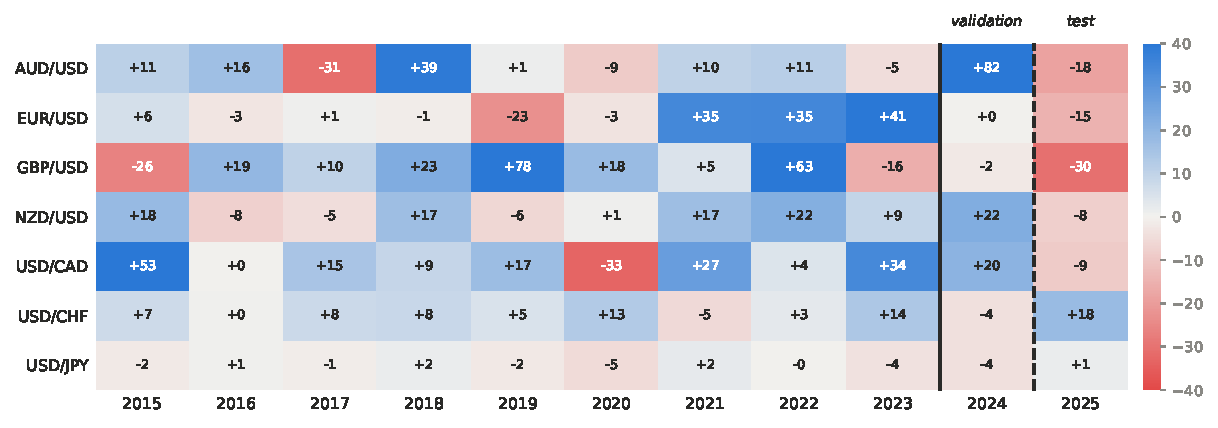
\includegraphics[width=\textwidth]{Images/YearlyExcess.pdf}
\caption{Yearly return of each agent minus the return of buying and holding the same pair, in percentage points. Blue is outperformance. The solid line marks the end of the training data and the dashed line the end of the validation year, so only the last column was unseen by any part of the procedure.}
\label{Figure:YearlyExcess}
\end{figure}

There is a market explanation for the direction of the 2025 result, and it is worth giving because it points somewhere. 2025 was a broad dollar reversal: EUR/USD rose $13.5\%$, its largest annual move in the eleven years, and the dollar weakened against five of the seven pairs. The agents were trained on a decade in which the dollar mostly strengthened, and six of the seven were positioned for that. The seventh, USD/CHF, is the least directional model in the set, holds the fewest positions and has the lowest beta, and it is the one that made money. That is consistent with the rest of the evidence rather than a coincidence: the model that depends least on a market direction is the one that survived the direction changing.

The individual results are worth reading rather than only their average, because they do not fail in the same way. GBP/USD is the worst at $-22.9\%$, and it is the most aggressive model in the set, running near full size with the deepest drawdown over the full window; a year that goes against it costs accordingly. USD/CAD loses $13.4\%$ and AUD/USD $11.7\%$, and both are the leveraged-exposure models of Section~\ref{Subsection:AlphaBeta}, so a reversal in the direction their beta points is exactly the event that hurts them. EUR/USD loses only $1.2\%$ despite the pair moving $13.5\%$, which is consistent with its near-zero beta: it did not participate in the reversal in either direction.

The two that held up are the two that were holding least. USD/CHF returned $+5.0\%$ while its pair fell $12.8\%$, an excess of $17.8$ percentage points and its best year against the benchmark in the whole sample. USD/JPY returned $+0.6\%$, which is not skill but the absence of exposure to the pairs that moved. Between them they describe the pattern: the models that depended least on a market direction were the ones that survived the direction changing.

One year is a small sample and no conclusion should be drawn from it beyond the obvious one. What the held-out year establishes is a bound, not a verdict: the design continued to trade sensibly on data it had never seen, and it lost money doing so in a year whose direction its training data did not contain.